\chapter{Related Work}

\section{\citefield{sggx}{title}}
Since we represent our \acp{lod} as volumes choosing a phase function is required to compute the scattering directions in the medium.
We choose the SGGX phase function because it has similar scattering properties as the GGX \ac{brdf}\cite[p. 2]{sggx}.
The idea behind the GGX \ac{brdf} and other microfacet models is that a surface can be modeled by a distribution of normals which describe the roughness of the surface at a certain point \cite[p. 3]{ggx}.
Expanding on this idea \citeauthor{microflake} introduced the microflake framework which models the medium as two-sided specularly reflecting flakes which are distributed according to a certain \ac{ndf} \cite[pp. 4-5]{microflake}.
\citeauthor{sggx} define the \ac{ndf} for the SGGX phase function as:
\begin{equation}
    D(\omega_m)=\frac{1}{\pi \sqrt{|S|}(\omega_m^T S^{-1} \omega_m)^2},
\end{equation}
where $\omega_m$ is the direction of the microflake normal and $S$ is a 3 $\times$ 3 symmetric positive definite matrix which encodes the scattering properties \cite[p. 4]{sggx}.
This \ac{ndf} can be seen as the extension of the GGX \acs{ndf} to the negative hemisphere:
\begin{figure}[!ht]
    \centering
    \begin{subfigure}[b]{0.45\linewidth}
        \centering
        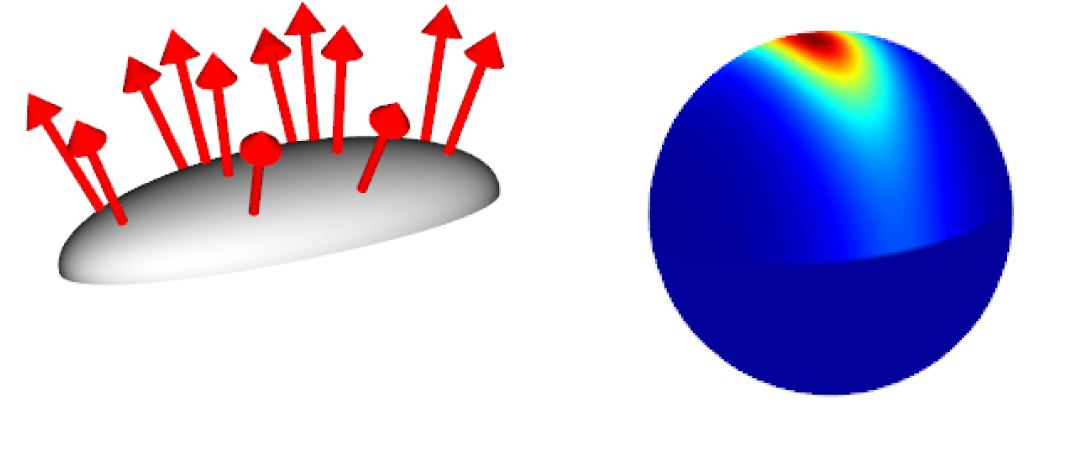
\includegraphics[width=\linewidth]{img/sggx_ndf_a.jpg}
        \caption{GGX $D(\omega_m), \omega_m \in \Omega^+$ \cite[p. 3]{sggx}}
        \label{fig:sggx_ndf_a}
    \end{subfigure}
    \begin{subfigure}[b]{0.45\linewidth}
        \centering
        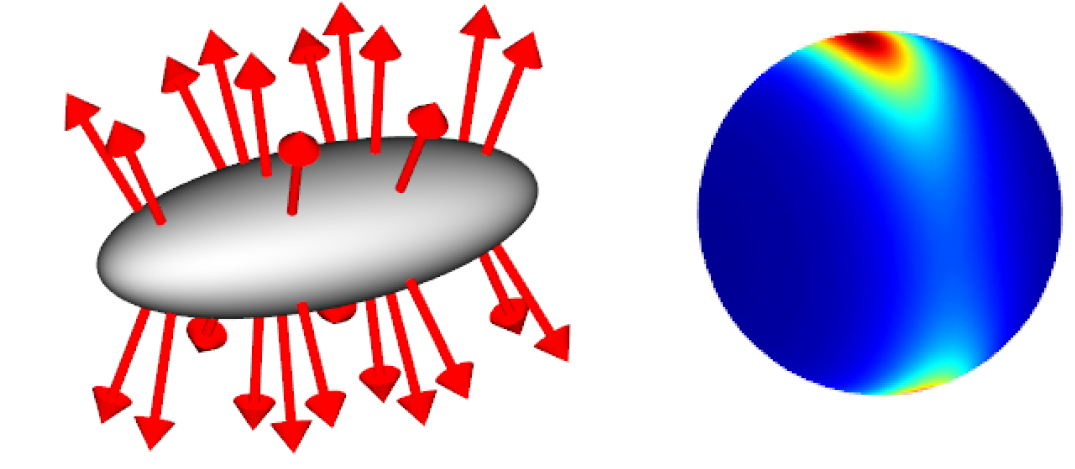
\includegraphics[width=1\linewidth]{img/sggx_ndf_b.jpg}
        \caption{SGGX $D(\omega_m), \omega_m \in \Omega$ \cite[p. 3]{sggx}}
        \label{fig:sggx_ndf_b}
    \end{subfigure}
	\caption{Visualization of anisotropic \acsp{ndf}. Note that the negative hemisphere of the SGGX \acs{ndf} is a mirroring of the positive hemisphere.}
	\label{img:sggx_ndf}
\end{figure}
Based on the \acs{ndf} the authors then introduce a \ac{vndf} $D_{\omega_i}(\omega_m)$ which is used for importance sampling of the phase function, since it reduces variance as opposed to the \acs{ndf} \cite[p. 9]{vndf_importance_sampling}.
Another important concept in the mikroflake framework is the projected area $\sigma(\omega_i)$ of the microflakes.
This is the area of the microflakes when projected onto a plane in direction $\omega_i$ \cite[p. 3]{sggx}.
\begin{figure}[!ht]
    \centering
    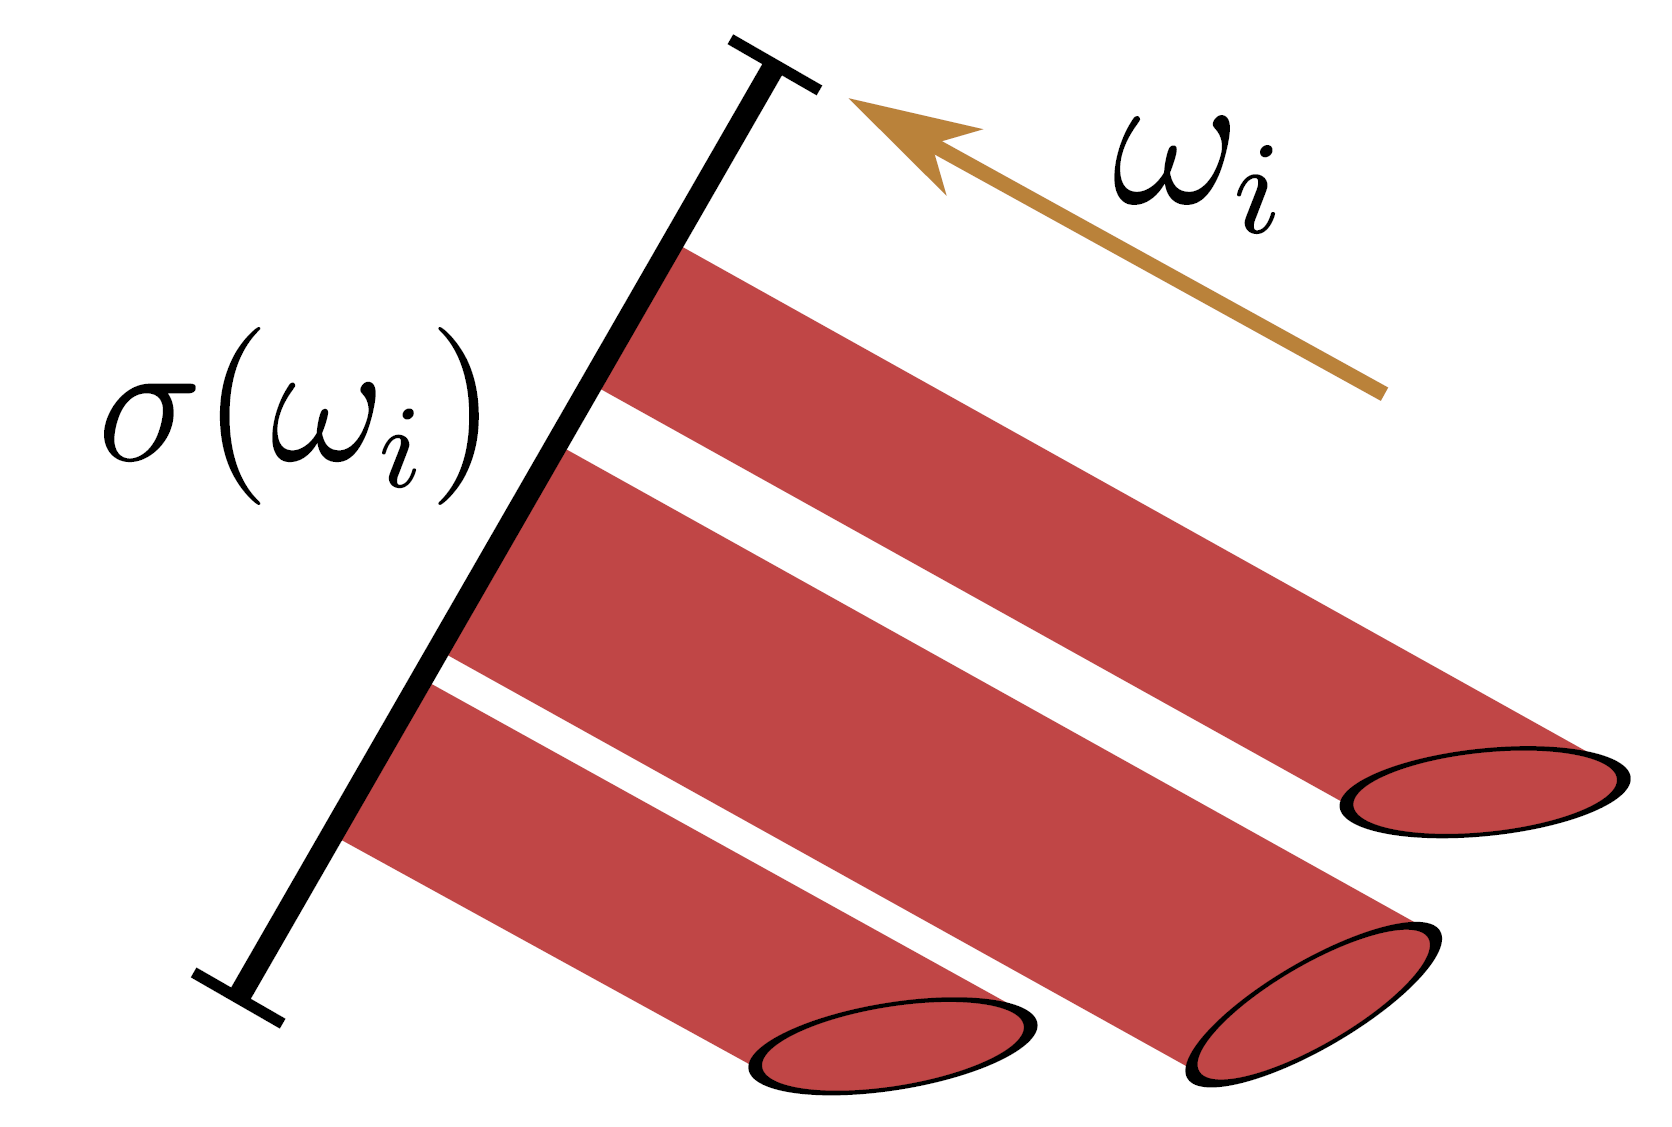
\includegraphics[width=0.3\linewidth]{img/sggx_projected_area.png}
    \caption{Projected area $\sigma(\omega_i)$ \cite[p. 2]{sggx}.}
    \label{fig:sggx_projected_area}
\end{figure}
For the SGGX phase function the projected area is defined as \cite[p. 4]{sggx}:
\begin{equation}
    \label{eq:projected_area}
    \sigma(\omega_i)=\int_\Omega \langle \omega_i, \omega_m \rangle D(\omega_m) d\omega_m = \sqrt{\omega_i^T S \omega_i},
\end{equation}
where $\langle -,-\rangle$ denotes the clamped dot product \cite[p. 3]{sggx}.
Having defined these terms the authors introduce the actual phase function which consists of a specular and a diffuse component.
The specular component is evaluated as \cite[p.7]{sggx}:
\begin{equation}
    f{}^{spec}_p(\omega_i \rightarrow \omega_o) = \frac{D(\omega_h)}{4 \sigma(\omega_i)}.
\end{equation}
Importance sampling the specular component requires to sample a normal from $D_{\omega_i}$ and the direction $\omega_i$ is reflected on this normal to generate an outgoing direction $\omega_o$ \cite[p. 8]{sggx}.
For evaluating the diffuse phase function \citeauthor{sggx} propose to sample a normal $\omega_m$ from $D_{w_i}$ which gives an unbiased estimate of the following integral \cite[p. 8]{sggx}:
\begin{equation}
    f{}^{diff}_p(\omega_i \rightarrow \omega_o) = \frac{1}{\pi}\int_\Omega \langle\omega_o,\omega_m\rangle D_{\omega_i}(\omega_m) d\omega_m = \lim \limits_{N \to +\infty} \frac{1}{N} \sum_{n=1}^N \frac{1}{\pi} \langle\omega_o,\omega_m(n)\rangle.
\end{equation}
$f{}^{diff}_p$ can then be importance sampled by generating a direction $\omega_m$ from $D_{\omega_i}$ and then sampling the hemisphere given by $\omega_m$ \cite[p. 8]{sggx}.

\section{\citefield{hybrid_mesh_volume_lods}{title}}
Another important paper for the thesis is \citetitle{hybrid_mesh_volume_lods} by \citeauthor{hybrid_mesh_volume_lods}.
Their idea is to represent macroscopic surfaces (larger than the target resolution) as mesh \acsp{lod} while microscopic geometry (smaller than the target resolution) is represented in volumes \cite[p. 3]{hybrid_mesh_volume_lods}.
This is different to our approach as we represent both cases by volumes.
The first step in their pipeline is to seperate the macroscopic from the microscopic geometry \cite[p. 5]{hybrid_mesh_volume_lods}.
For a tree that would mean to seperate the trunk from the branches and leafs \cite[p. 3]{hybrid_mesh_volume_lods}.
The second step is to apply mesh simplification on the macroscopic surface while preserving the reflectance properties.
They achieve mesh simplification by using edge collapse, therefore they remove triangle edges which are smaller than the target resolution.
The adjacent triangles collapse as a result as well \cite[p. 6]{hybrid_mesh_volume_lods}.
To preserve reflectance the authors update the diffuse and specular albedos of the remaining vertices by a weighted sum of the old vertices \cite[p. 6]{hybrid_mesh_volume_lods}.
The last step in their pipeline is the voxelization of the sub-resolution geometry.
The authors choose a ray casting approach to estimate the density for each voxel \cite[p. 8]{hybrid_mesh_volume_lods}.
To sample ray origins the authors use a \ac{pdf} $D_i=D_i^{cube} \ast D^{smooth}$ around the voxel center \cite[p. 9]{hybrid_mesh_volume_lods}.
$D_i^{cube}$ is a cubic uniform \ac{pdf} around the voxel center and $D^{smooth}$ is a 3D gaussian function with the standard deviation of 0.6 times the length of the voxel edge \cite[p. 9]{hybrid_mesh_volume_lods}.
The length of the rays is set to the length of the voxel edge \cite[p. 9]{hybrid_mesh_volume_lods}.
We deviate from this ray generation procedure as we choose the ray origin on a cubic uniform \ac{pdf} around the voxel center and clip our rays at a bounding sphere around the voxel.
Details to our procedure are explained in section \dots.
Each ray is intersected with the micro-geometry, the number of hits and the total number of rays casted determine the occlusion probability \cite[p. 8]{hybrid_mesh_volume_lods}:
\begin{equation}
    P_{occ}=\frac{nbHits}{nbRays}.
\end{equation}
Since a medium is defined on the density $\rho$ the authors solve the integral
\begin{equation}
    1 - \frac{1}{4\pi}\int_\Omega e^{-\rho\sigma_u(\omega)ray_l} d\omega = P_{occ}
\end{equation}
for $\rho$ \cite[p. 9]{hybrid_mesh_volume_lods}.
$\sigma_u(\omega)$ is the microflake projected area as defined in \ref{eq:projected_area} and $ray_l$ is again the length of the voxel edge.
This equation cannot be solved analytically and therefore requires gradient descent based optimization of $\rho$ \cite[p. 9]{hybrid_mesh_volume_lods}.
In section \dots we further explore this optimization procedure.

% \section{\citefield{brick_grid}{title}}
\section{\citetitle{brick_grid}}
The paper \citetitle{brick_grid} by \citeauthor{brick_grid} is also highly relevant for the thesis as it provides optimization procedures to the standard null-collision methods used in heterogeneous media.
Required for null-collision methods is a density majorant in order to homogenize the medium.
Having such a majorant it is possible to sample distances as if the medium was homogeneous \cite[p. 3]{brick_grid}.
\begin{figure}[!ht]
    \centering
    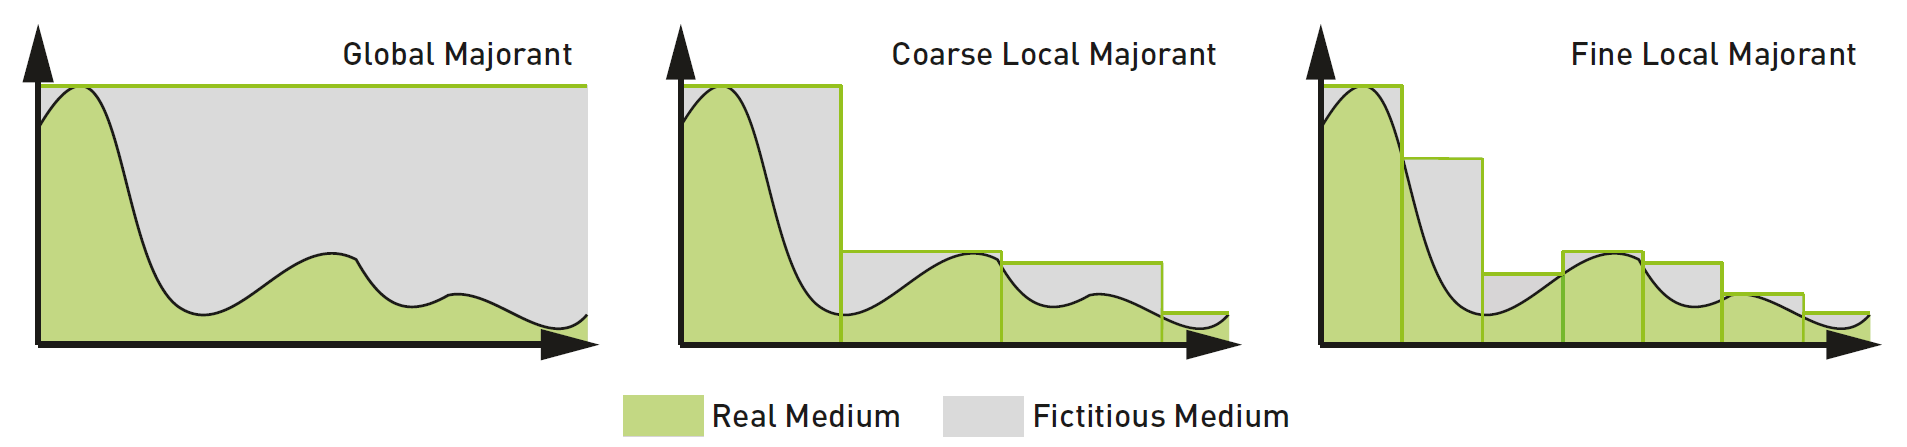
\includegraphics[width=0.9\linewidth]{img/brick_grid_majorants.png}
    \caption{Visualization of the concept of local majorants. These allow to sample distances and estimate transmittance more efficiently \cite[p. 3]{brick_grid}.}
    \label{fig:brick_grid_datastructure}
\end{figure}
Although this gives an unbiased result it may be inefficient to sample distances in this way when the density of the medium varies strongly.
Therefore the authors use local majorants which are valid in parts of the medium \cite[p. 3]{brick_grid}.

To store the volume data three textures are used.
First they use an \textit{atlas texture} to store \textit{bricks} which are groups of $8 \times 8 \times 8$ voxels \cite[p. 4]{brick_grid}.
The second texture is the \textit{indirection texture} which stores offsets into the atlas.
This texture therefore links a position in space to a brick of data in the atlas \cite[p. 4]{brick_grid}.
Finally \citeauthor{brick_grid} store the minorant and majorant of each brick in the \textit{range texture} \cite[p. 4]{brick_grid}.
These are used to scale the density values in the atlas texture to the interval $[0, 1]$ \cite[p. 4]{brick_grid}.
The range texture additionally has three mipmap levels which allows to have local majorants at different scales \cite[p. 7]{brick_grid}.
\begin{figure}[!ht]
    \centering
    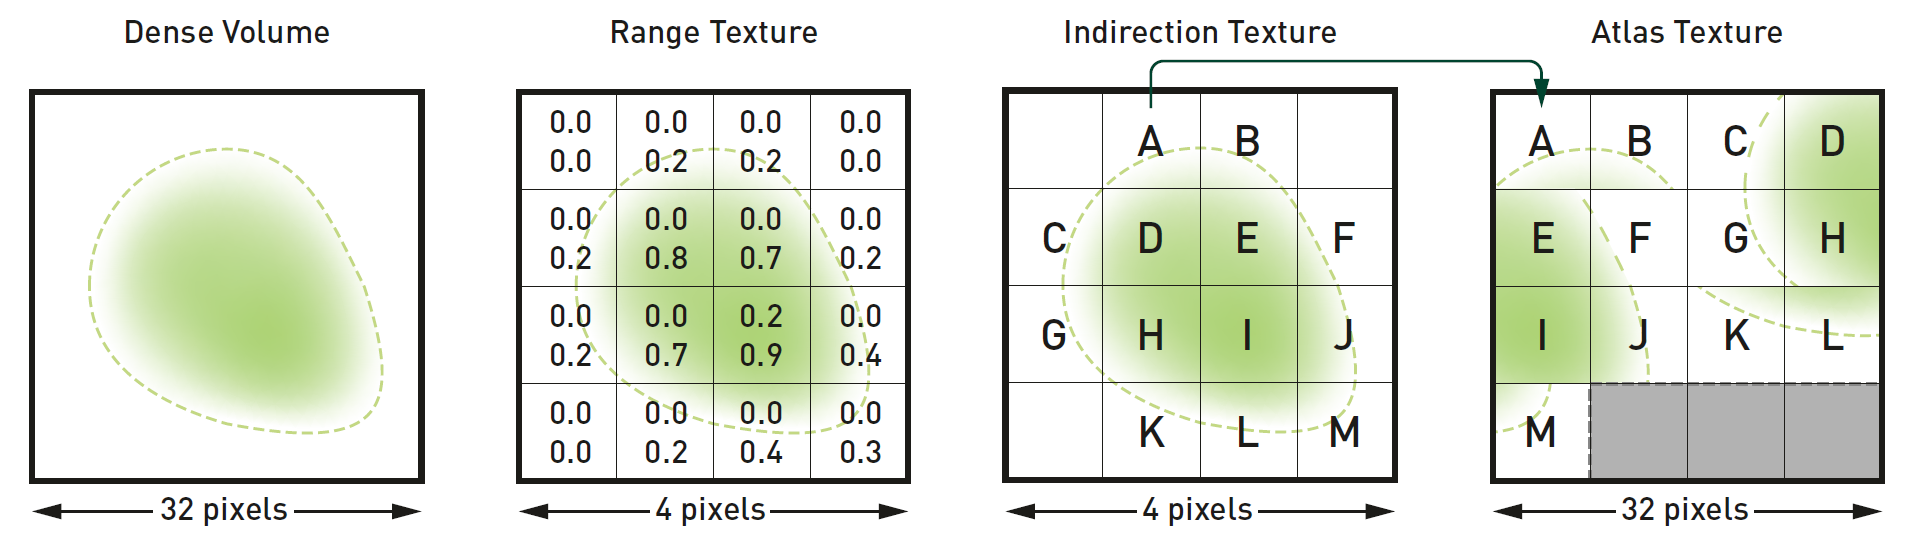
\includegraphics[width=0.9\linewidth]{img/brick_grid_datastructure.png}
    \caption{Datastructure of brick grid \cite[p. 4]{brick_grid}.}
    \label{fig:brick_grid_datastructure}
\end{figure}
Since the resulting atlas texture no longer has spatial coherence hardware interpolation by the texture unit is not possible \cite[p. 5]{brick_grid}.
Therefore the authors employ a form of stochastic lookup where they jitter the lookup point by $\pm0.5$ voxels before doing point sampling \cite[p. 5]{brick_grid}.
When having a large number of lookups, as it is the case in Monte Carlo integration, this is equivalent to trilinear interpolation without introducing a significant overhead \cite[p. 5]{brick_grid}.
For distance sampling and transmittance estimation \citeauthor{brick_grid} first sample a target optical thickness $\tau_{target}=-ln(1-\xi)$ \cite[p. 6]{brick_grid}.
They then accumulate the optical thicknesses of all bricks along a ray until the accumulated thickness exceeds the target thickness \cite[p. 6]{brick_grid}.
In this case they step back along the ray until it matches $\tau_{target}$ \cite[p. 6]{brick_grid}.
Now they perform the stochastical null-collision test by comparing the density at this point with the local majorant \cite[p. 6]{brick_grid}.
In the case of distance sampling, they return the distance to the first real collision \cite[p. 6]{brick_grid}.
For transmittance estimation, they adjust the current estimate by the ratio of real to fictious matter \cite[p. 6]{brick_grid}.
When having a null-collision, the algorithm is restarted by sampling a new target optical thickness \cite[p. 6]{brick_grid}.
This is repeated until a distance is successfully sample, the transmittance estimation is ended by russian roulette or the ray left the volume \cite[p. 6]{brick_grid}.